%   Filename    : chapter_4.tex 
\chapter{Preliminary Results/System Prototype}
This chapter presents the preliminary results of the study, including findings from data gathering, the system's diagrams and designs, initial user interface (mockup UI) for the front end, and the chatbot's architecture.

\section{Data Gathering Results}
The research process for developing TUKIB started with a comprehensive visit to the UPV RRC during the researchers' internship. This phase involved engaging with key personnel and understanding the intricacies of the center's operations. The following sections detail the key activities and information undertaken and gathered during this visit.

\subsection{Facility Tour}
During the researcher's visit, they met with the center's director, administrative staff, and laboratory heads. This introduction provided valuable insights into the roles and responsibilities of various individuals and departments within the RRC. Understanding these dynamics was crucial for tailoring the system to fit the center’s workflows.

The researchers were also given a guided tour, which provided an overview of various laboratories and services offered. These services includes:

\begin{itemize}
	\item \textbf{Sample Processing.}The RRC provides critical sample processing services, essential for research and analysis.
	\item \textbf{Laboratory Equipment Rental} Various pieces of laboratory equipment are available for rent, which supports a wide range of scientific projects.
	\item \textbf{Training and Workshops.} The RRC offers training sessions on laboratory equipment, promoting user proficiency.
	\item \textbf{Facility Rentals.} Access to spaces like the Audio-Visual Room (AVR) and conference rooms was noted as a valuable resource for users.
\end{itemize}

Each laboratory, including the Biology, Microbiology, Nanotechnology, and Applied Chemistry labs, was introduced in detail, with specific equipment and services discussed in terms of their availability and purpose. The UPV RRC houses five (5) laboratories, namely: Biology, Microbiology, Nanotechnology, Applied Chemistry Laboratory, and Food, Feeds, and Functional Nutrition Laboratory.

\subsection{Stakeholder Identification and Engagement}
The success of workflow automation hinges on understanding the needs and expectations of its key stakeholders. These stakeholders include the RRC laboratory and administrative staff, the clients (university and student researchers and external users of the RRC facilities), the developers, and the member/s of the Computer Science Faculty guiding the project.

The researcher's interaction with the stakeholders allowed them to gather valuable feedback on the existing system and the challenges they faced. This feedback played a crucial role in shaping the direction of our system design, as it highlighted the need for automation, service tracking, and streamlined communication between stakeholders. Additionally, stakeholders were interviewed on their specific needs and pain points. These discussions led to the creation of user stories, which helped to contextualize the requirements from various perspectives. 

This in-depth exposure to the center’s operations was essential for the initial design and development phase of TUKIB, providing a strong foundation for creating a system tailored to the specific needs of the RRC and other research institutions with similar setups.

\subsection{Scope and Limitations of the Services}
Through direct discussions with the center’s director and administrative staff, the researchers obtained a clear picture of the scope of services provided by each facility, as well as the current limitations they face. Some of these limitations include:

\begin{itemize}
	\item The UPV RRC currently has no centralized system available to the public which describes its mission, vision, services offered, as well as, steps on how to request a service, and other relevant information. This limits clients from acquiring necessary information about the center and its services.
	\item The staff also has difficulty in tracking equipment and facility availability in real-time, as it is essential to ensure that no one else is using an equipment or facility before it can be rented out on a specific time and date.
	\item Manual service request and data management are also a problem as the RRC’s current system relies mainly on Google Forms and Sheets, which poses challenges in efficiency and scalability.
\end{itemize}

\subsection{User Requirements}

Based on the gathered data with stakeholders and observations during the facility tour, several key user requirements were identified for the development of TUKIB. 

\begin{itemize}
	\item \textbf{Service Information Accessibility}
	\item \textbf{Automated Service Requests}
	\item \textbf{Equipment and Facility Availability Tracking}
	\item \textbf{Data Management and Reporting}
	\item \textbf{User Account Management}
	\item \textbf{Feedback Mechanism.}
\end{itemize}
\newpage

\section{System Design}

\subsection{Process Flow Diagram}

\begin{figure}[h]
	\centering 
	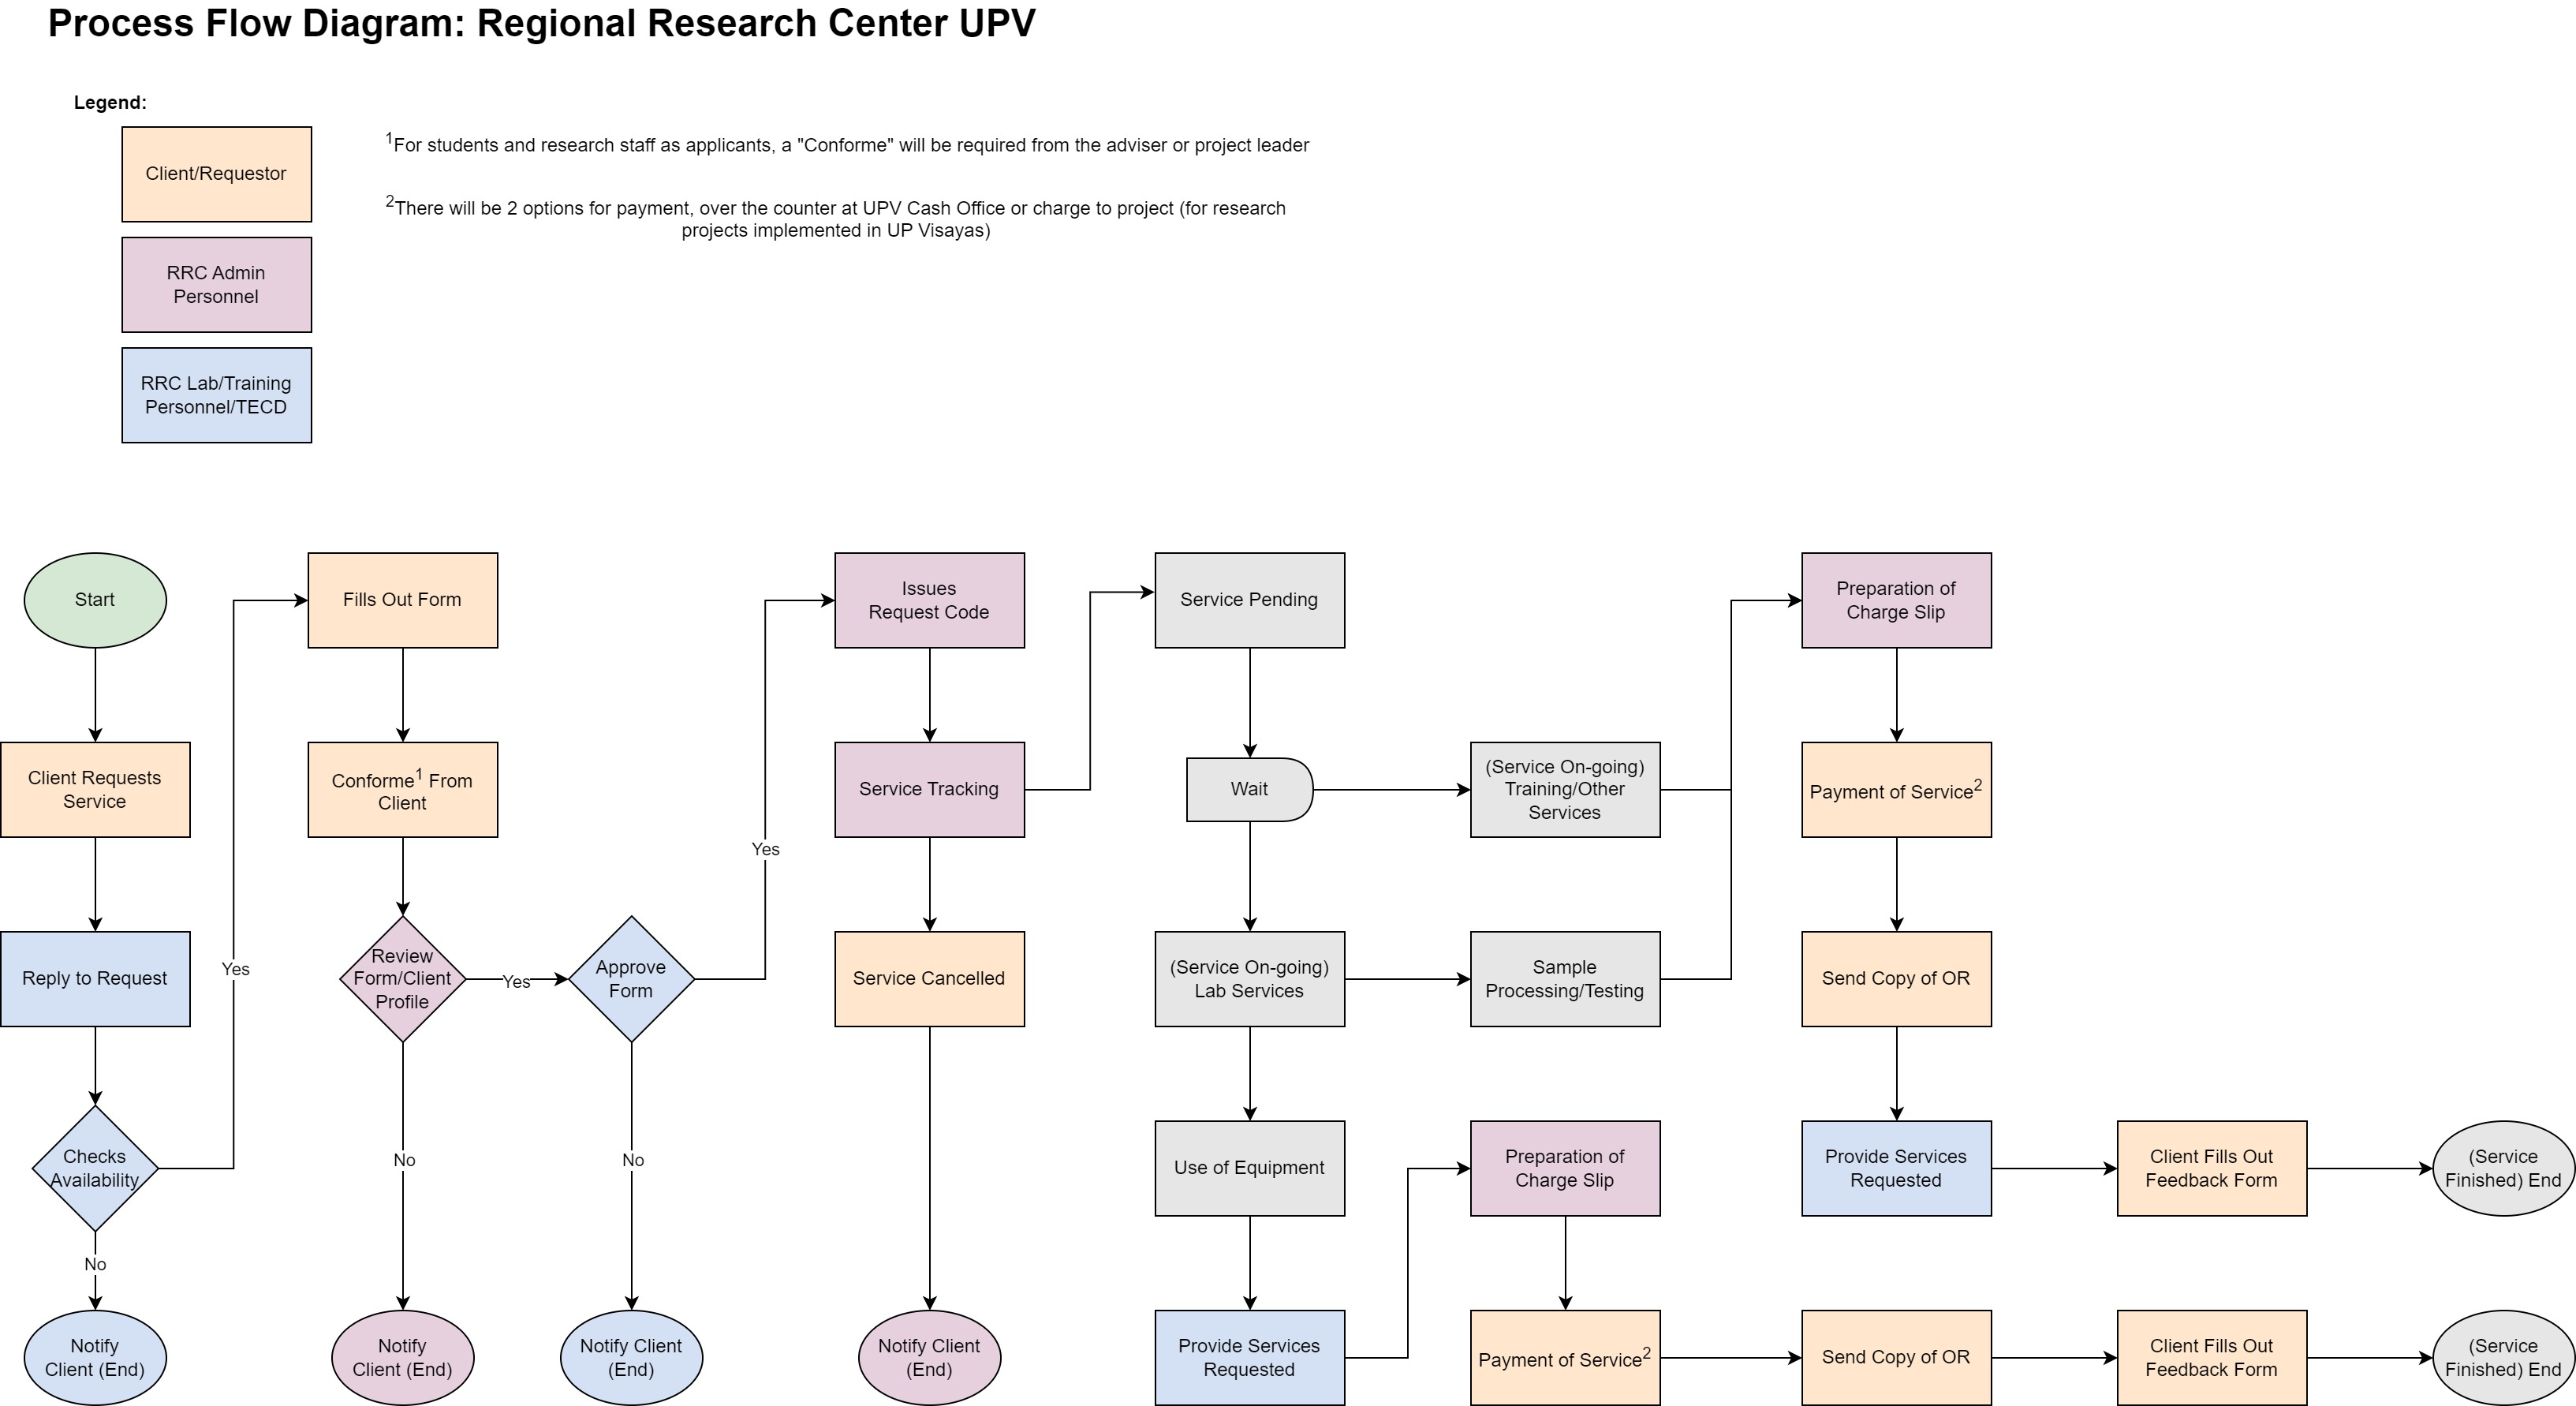
\includegraphics[width=1\textwidth]{process_flow.jpg}
	\caption{Process flow diagram from service request to feedbacking}
	\label{fig:process_flow}
\end{figure}

\figref{fig:process_flow} illustrates the entire service delivery process of RRC. The process starts with a service request from the client and ends with a feed back from them.

\newpage

\subsection{Context Model}

\begin{figure}[h]
	\centering 
	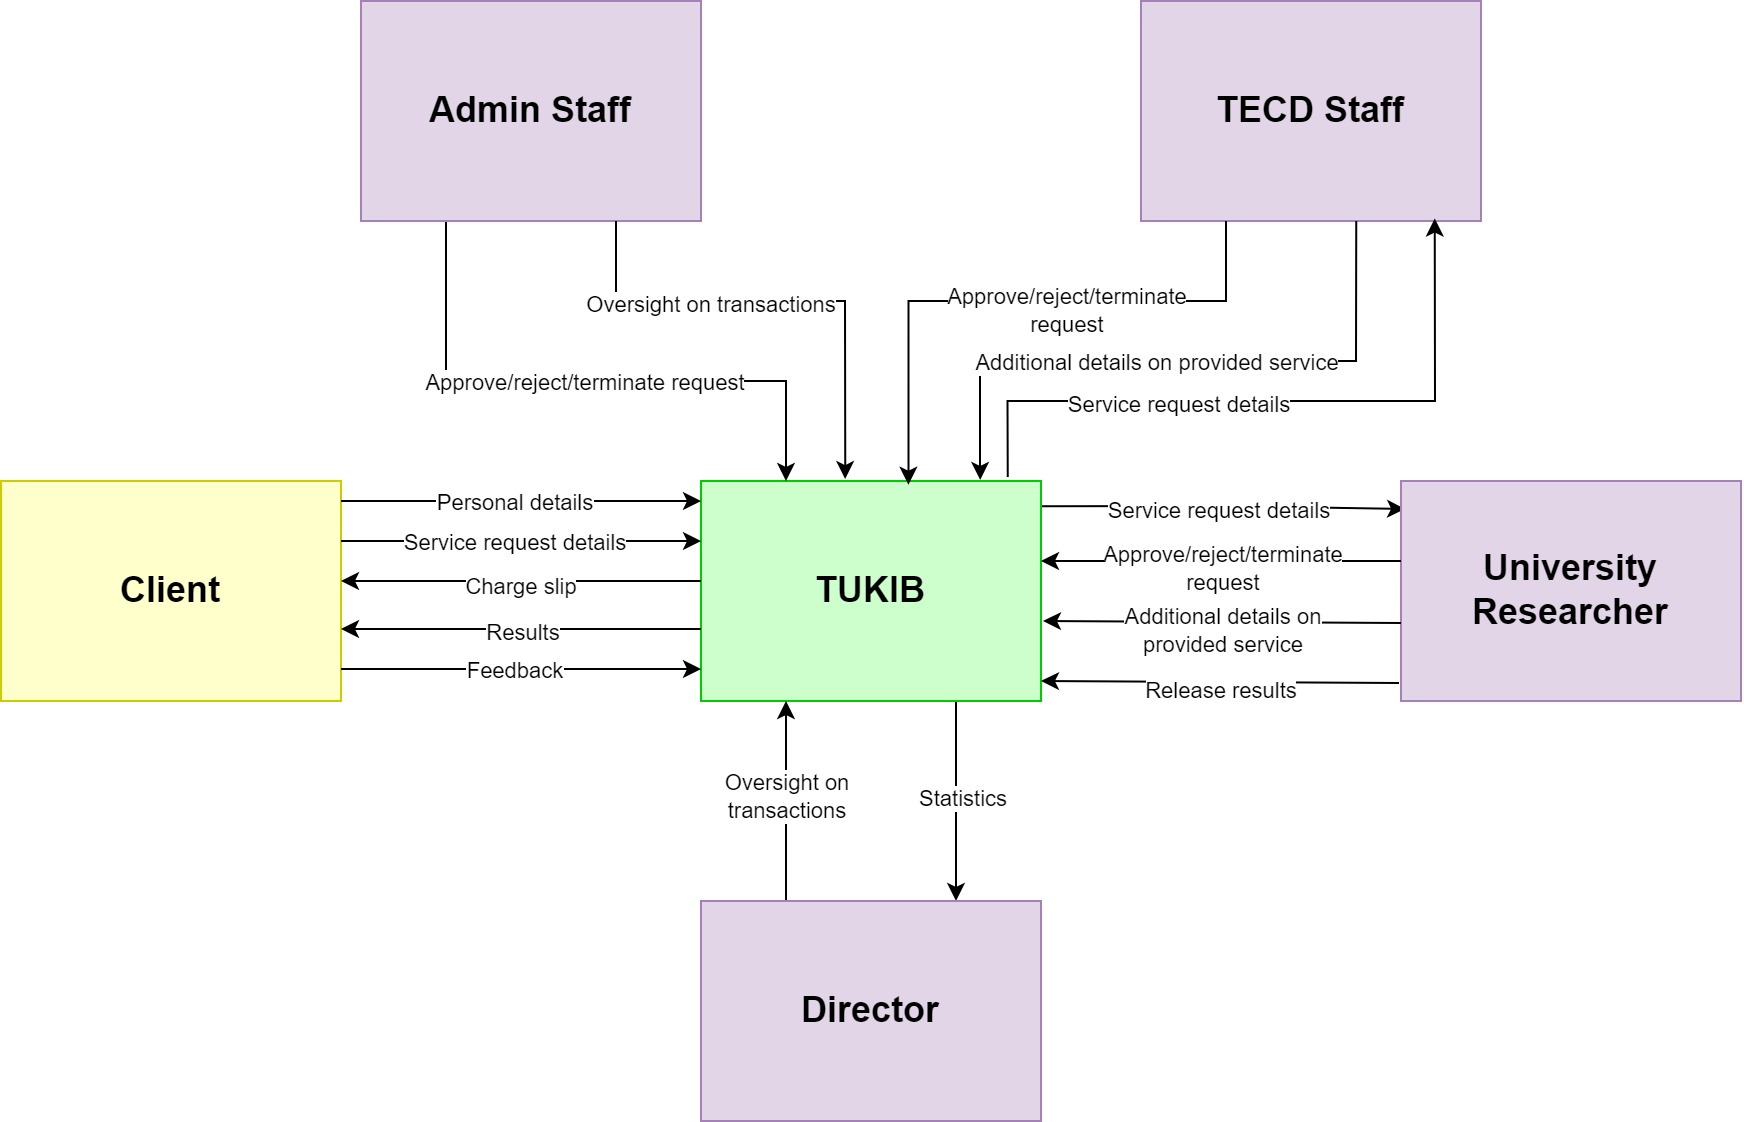
\includegraphics[width=0.9\textwidth]{context model.png}
	\caption{Context model for interactions between the TUKIB and its users}
	\label{fig:context_model}
\end{figure}

\figref{fig:context_model} illustrates the interactions between the system and both internal and external entities. It highlights how the system communicates with different stakeholders, including client, staff, director, and university researcher. The model also outlines how information flows entities to the system and vice versa, showing how the system works and its role within the institution.

\newpage

\subsection{Data Flow Diagram}

\begin{figure}[h]
	\centering 
	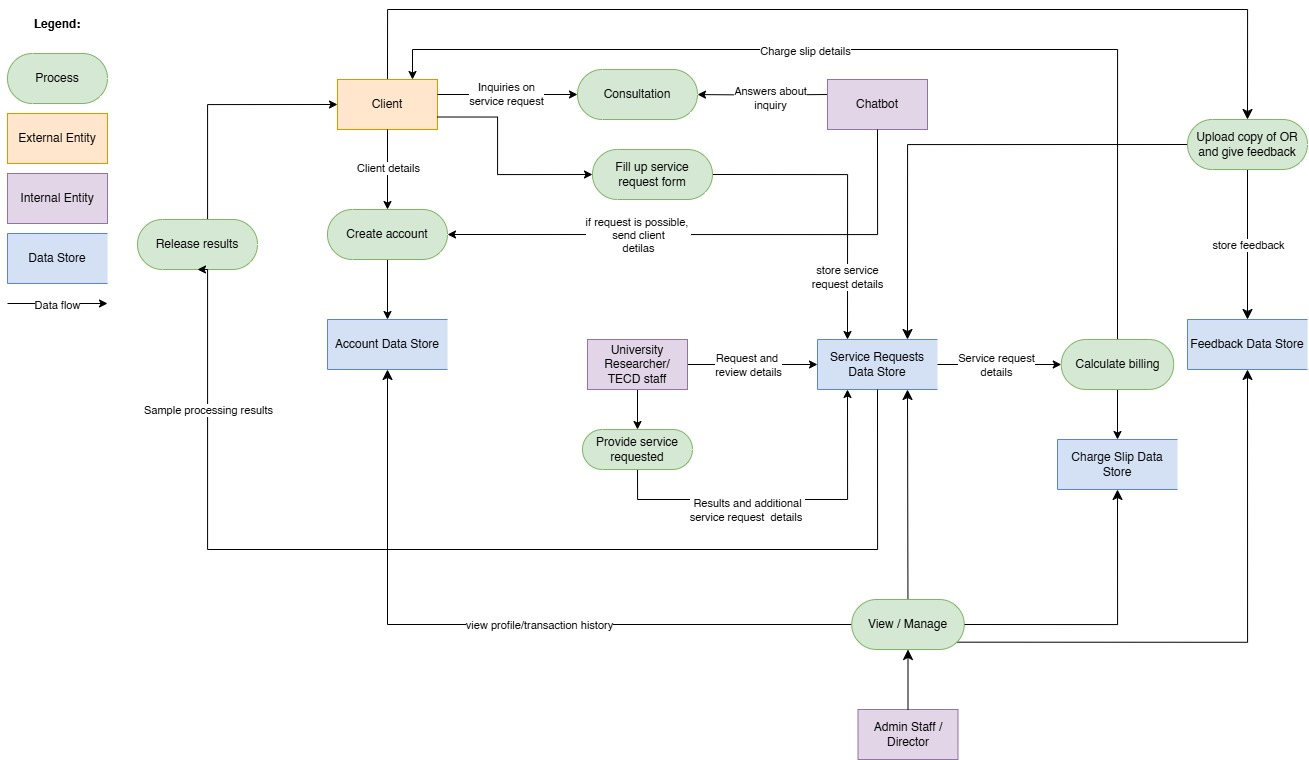
\includegraphics[width=1\textwidth]{data_flow.jpg}
	\caption{Data flow diagram from service request to feedbacking}
	\label{fig:data_flow}
\end{figure}

\figref{fig:data_flow} shows the flow of data within the system, illustrating how information is exchanged between different components and users. The diagram also illustrates the pathways through which data moves, providing overview into how information are stored and retrieved within the system.

\newpage

\subsection{Database Diagram}

Figure something illustrates the database diagram of the system.

\newpage

\section{Chatbot}

\textbf{Entities and Intents}

From the data gathering phase, the developers were able to identify common user queries and specific service requirements needed for the development of the chatbot. The collected data was used to construct the intents and entities which are essential for the chatbot’s functionality. 

Intents represent the goal the users want to achieve when interacting with the chatbot (e.g., ”start consultation,” ”ask about lab rental procedures,” ”inquire about service status”). The intents are divided into greeting, general, service requests, frequently asked questions, feedback, and end or closing message. 

On the other hand, entities are specific pieces of information that the chatbot needs to get from the user in order to fulfill a task. For example, the chatbot needs to know the laboratory name and desired time for renting the equipment in order to indicate its availability. 

\newpage

\noindent \textbf{Conversation Flow}

\begin{figure}[h]
	\centering 
	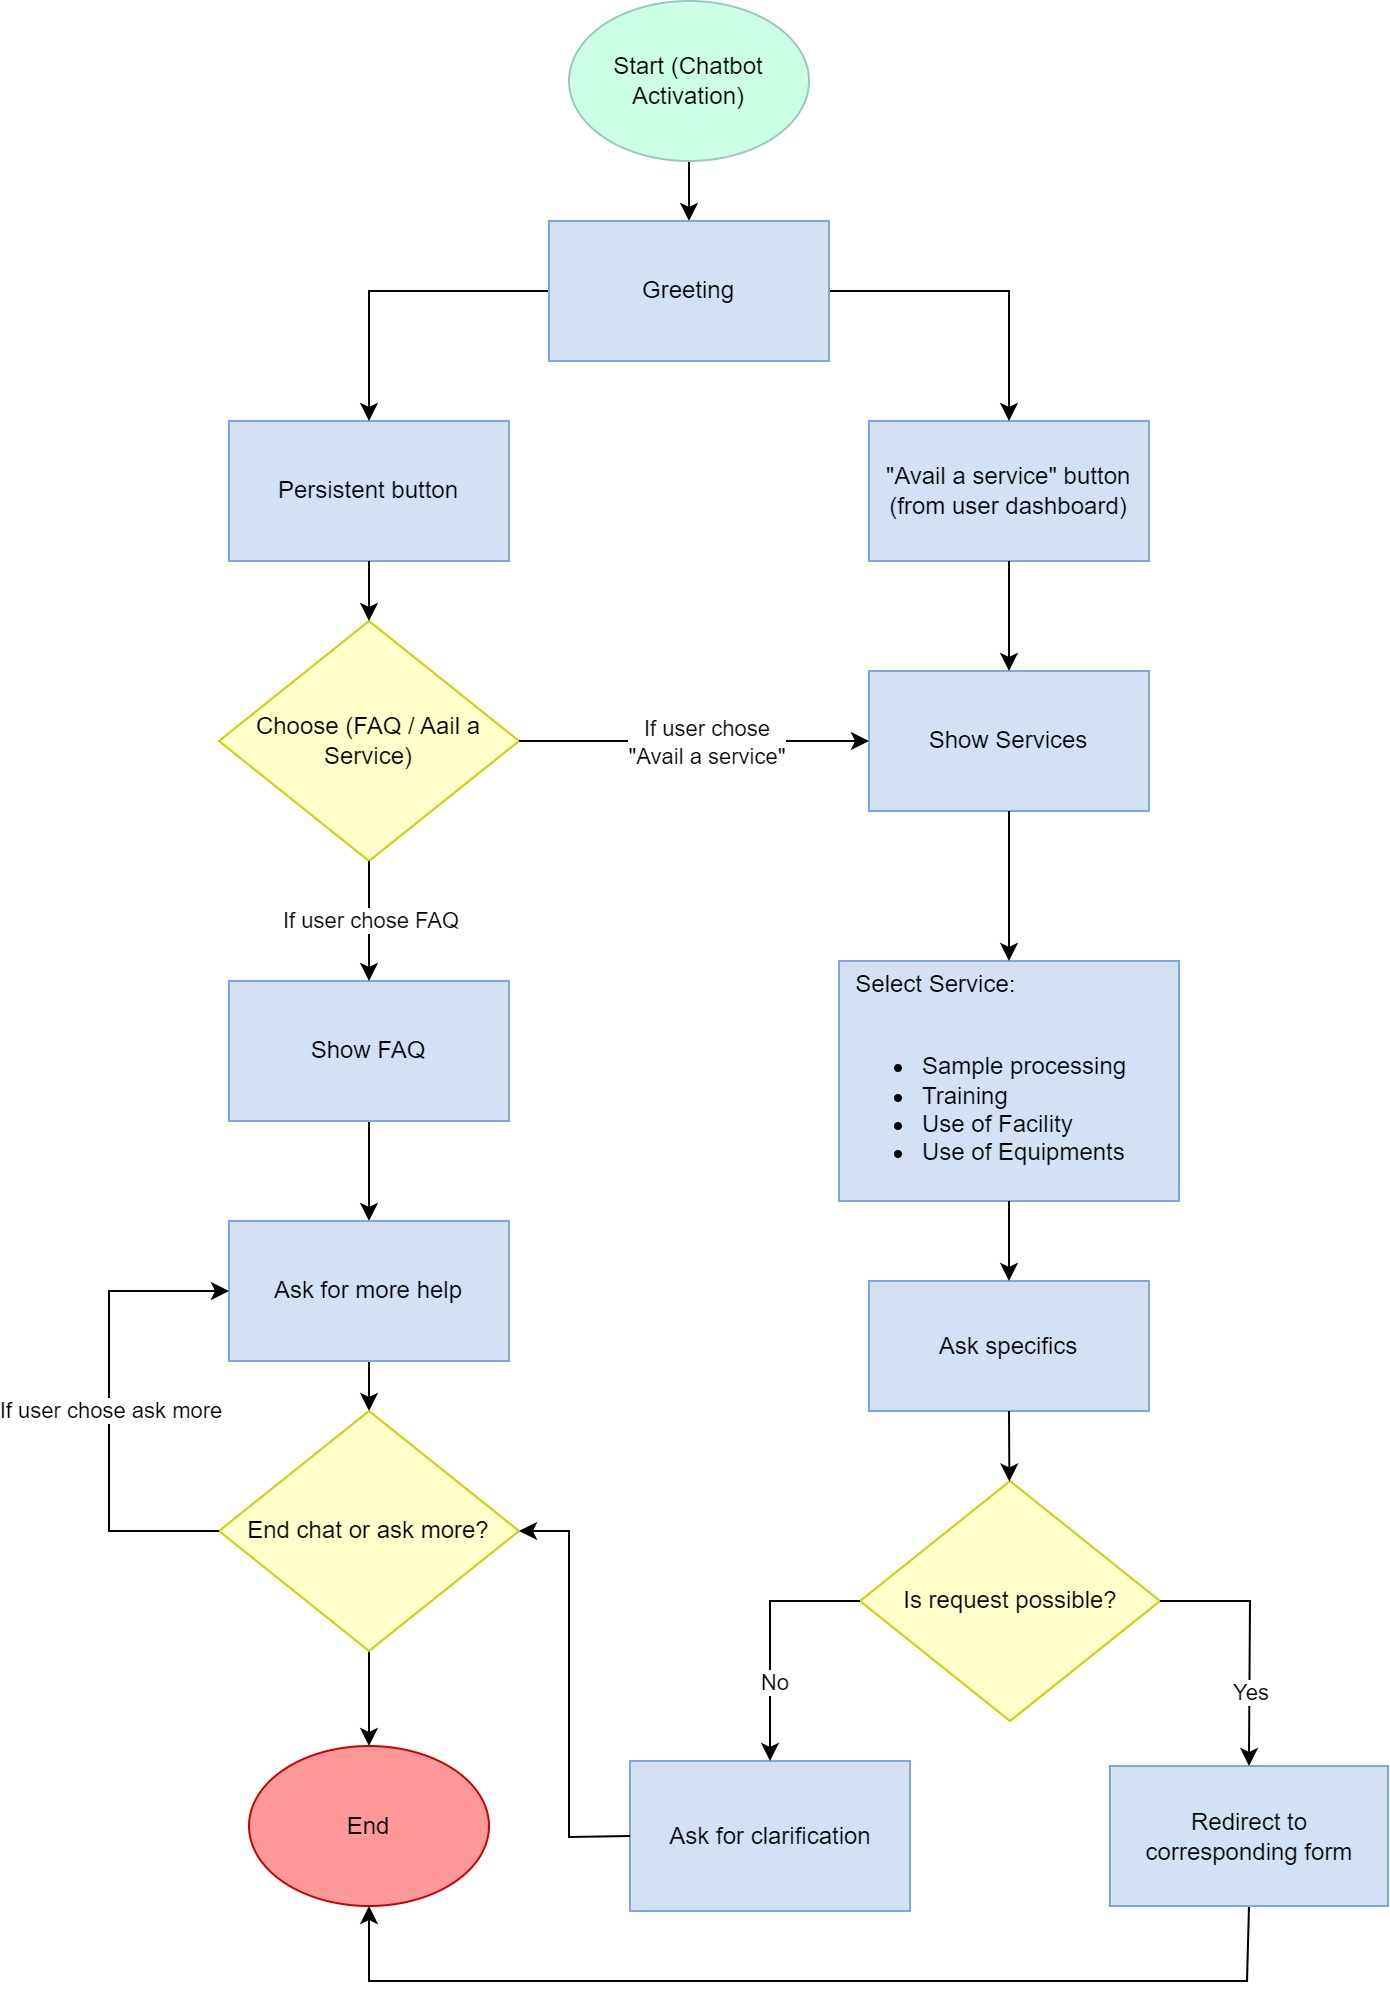
\includegraphics[width=0.7\textwidth]{chatbot_flow.jpg}
	\caption{LIRA conversation flow}
	\label{fig:chatbot_flow}
\end{figure}

\figref{fig:chatbot_flow} illustrates the conversation flow for TUKIB's chatbot, named LIRA— short for Learning, Innovation, and Research Assistant. LIRA will be accessible throughout the entire website, ensuring that all users, whether logged in or not, can obtain support whenever needed. Users can initiate a chat with LIRA via a persistent button that remains visible across the site or by selecting the dedicated “Avail a Service” button found on the user dashboard.

The architecture of the chatbot is centered around a conversational flow that guides users through various tasks, from inquiries to service requests. The chatbot’s design consists of the following core components:

\begin{itemize}
	\item \textbf{Welcome Greeting}
	
	\subitem Present a welcome message where the chatbot greets users with a friendly introduction and offers assistance, presenting options such as “Service Inquiry“ and “Frequently Asked Questions/FAQs”
	
	\item \textbf{Flow for Service Inquiry}
	
	\subitem If the user chooses the option “Service Inquiry,” the chatbot will ask a follow-up question to identify which service the user wishes to inquire about. Sample service choices include sample processing,  lab equipment rental, etc. Then, the chatbot uses the user's answer details to present accurate information about each service. 
	
	\item \textbf{Flow for Consultation}
	
	\subitem The flow for consultation is designed to facilitate user inquiries about the services they wish to avail. As the primary purpose of the chatbot, this interaction allows users to ask questions about the services offered by RRC. When a user expresses interest, the chatbot engages by asking for specific details related to their request. For instance, if a user inquires about sample processing (e.g., the type of sample and processing methods needed), the chatbot will guide them through the details. This interactive process ensures that users receive tailored information while the chatbot gathers necessary details to asses service feasibility.
	
	\item \textbf{Flow for General Questions / FAQ}
	
	\subitem The chatbot should be able to answer and handle frequently asked questions by clients. These would include questions about general services, rental pricing methods, facility rental processes, etc.
	
	\item \textbf{Chatbot User Feedback}
	
	\subitem After chatbot services are completed, the chatbot will prompt the user to rate or provide feedback on their experience, which will help the developers and the RRC enhance their service quality.
	
	\item \textbf{Error Handling}
	
	\subitem Chatbot failures will lead to conversational dead ends if not dealt with properly. Thus negating the main purpose of chatbot in this system which is to provide efficient customer service. The chatbot will have a fallback mechanism whenever user input is unexpected or a system error occurs. For example, if the chatbot cannot understand the user input, there will be rules on how the chatbot would handle this situation. Sample fallback methods would be redirecting the conversation to a live agent. 
	
	\subitem Another option would be presenting friendly-toned error messages to the users, letting them know that the chatbot is having trouble understanding their input. Sample error messages would be “Sorry, I didn't catch that. Could you rephrase your question?” or “I'm sorry, I have a hard time understanding. Could you please rephrase your query?” and “I'm sorry, but what you're asking is not clear to me. Could you paraphrase it?” \newline
	
\end{itemize}


\section{User Interface Mock-up}

\subsection{Landing Page}

\subsection{User authentication and dashboard}

User dashboard is designed for the needs of two primary user groups of TUKIB who are the staff and clients. Each user group has a different user interface to cater to their specific needs. 

For the customers’ user interface, the developers designed a dashboard that shows the user’s profile, transaction history, and a button to avail a new service. For the staffs’ user interface, a layout was designed specifically for their tasks, featuring information and capabilities necessary for efficient management and oversight. This includes tools for monitoring workflows, accessing reports, and managing user requests.

The layout for both staff and customers’ user interface ensures easy navigation and quick access to essential information, enhancing the overall user experience.

